% ============================================================================
% SECTION: RESULTS - Global-APT Dataset
% ============================================================================
% To use in Overleaf:
% 1. Copy this file content into your LaTeX document
% 2. Add required packages in preamble (see below)
% 3. Adjust section numbering as needed
% 4. Convert Mermaid diagrams to TikZ or include as images

% ============================================================================
% REQUIRED PACKAGES (add to your preamble)
% ============================================================================
% \usepackage{booktabs}        % For professional tables
% \usepackage{multirow}        % For multirow cells
% \usepackage{graphicx}        % For figures
% \usepackage{tikz}           % For diagrams (optional)
% \usepackage{pgfplots}       % For plots (optional)
% \usepackage{siunitx}        % For number formatting

% ============================================================================
% SECTION: EXPERIMENTAL RESULTS
% ============================================================================
\section{Experimental Results}
\label{sec:results}

We evaluated several state-of-the-art anomaly detection algorithms on the Global-APT dataset, a temporal graph containing 4,632 events with 33.3\% labeled anomalies across 5 network nodes. The dataset was split chronologically into 70\% training, 15\% validation, and 15\% test sets.

\subsection{Dataset Characteristics}
\label{subsec:dataset}

The Global-APT dataset represents a small, highly centralized network with 5 nodes (IP addresses) and 4,632 temporal edges. The network structure exhibits strong centralization, with one hub node (172.16.0.50) receiving 75\% of all connections. This centralized structure, combined with the small number of nodes, creates a challenging environment for anomaly detection as most connection patterns appear frequent and "normal."

\subsection{Performance Comparison}
\label{subsec:performance}

Table~\ref{tab:results} presents the performance metrics for all evaluated algorithms. GraphSAGE achieved the best overall performance with a ROC-AUC of 0.97 and an F1-score of 0.86, successfully detecting 141 out of 142 anomalies (99.3\% recall) with only 44 false positives.

\begin{table}[htbp]
\centering
\caption{Performance comparison of anomaly detection algorithms on Global-APT dataset}
\label{tab:results}
\begin{tabular}{lcccccc}
\toprule
\textbf{Algorithm} & \textbf{ROC-AUC} & \textbf{Precision} & \textbf{Recall} & \textbf{F1-Score} & \textbf{TP} & \textbf{FP} \\
\midrule
GraphSAGE & \textbf{0.970} & 0.762 & \textbf{0.993} & \textbf{0.862} & 141 & 44 \\
SLADE & 0.556 & 0.344 & 0.996 & 0.511 & 235 & 449 \\
NetWalk & 0.662 & 0.356 & 0.993 & 0.524 & 141 & 255 \\
GAT & 0.521 & 0.337 & 1.000 & 0.504 & 142 & 279 \\
GeneralDYG & 0.494 & 1.000 & 0.004 & 0.008 & 1 & 0 \\
\bottomrule
\end{tabular}
\vspace{0.1cm}
\footnotesize
TP: True Positives, FP: False Positives. Test set contains 142 anomalies and 384 normal events.
\end{table}

\subsection{Key Findings}

\textbf{GraphSAGE outperforms all other methods} by achieving near-perfect anomaly detection (99.3\% recall) while maintaining high precision (76.2\%). This represents an excellent balance between detecting anomalies and minimizing false alarms, making it ideal for production deployment.

\textbf{SLADE, GAT, and NetWalk} all achieve near-perfect recall (99-100\%) but generate significantly more false positives. While these methods successfully identify almost all anomalies, their low precision (33-36\%) results in many false alarms that require manual review. This trade-off may be acceptable in security-critical applications where missing an anomaly is more costly than investigating false positives.

\textbf{GeneralDYG} performed poorly on this dataset, predicting almost all events as normal. This suggests the model requires significant hyperparameter tuning or may not be well-suited for small, highly centralized graphs.

\subsection{Threshold Optimization}

A critical finding was that default classification thresholds (0.5) led to poor performance, with some algorithms predicting all events as normal. We implemented automatic threshold optimization using F1-score maximization, which significantly improved results. For example, GraphSAGE's optimal threshold was 0.61 (vs. default 0.5), while GAT required a much lower threshold of 0.01 to achieve 100\% recall.

\subsection{Graph Structure Impact}

The small, centralized network structure (5 nodes, one hub receiving 75\% of traffic) explains why some algorithms struggle. With limited structural diversity, models learn primarily from frequency patterns, favoring the majority class (normal events). This highlights the importance of feature engineering and threshold optimization for small-scale temporal graphs.

% ============================================================================
% FIGURE: Network Structure (convert Mermaid to TikZ or include as image)
% ============================================================================
\begin{figure}[htbp]
\centering
% Option 1: Include as image (export Mermaid diagram as PNG/SVG)
% \includegraphics[width=0.8\textwidth]{figures/global_apt_graph.pdf}

% Option 2: TikZ diagram (manual conversion from Mermaid)
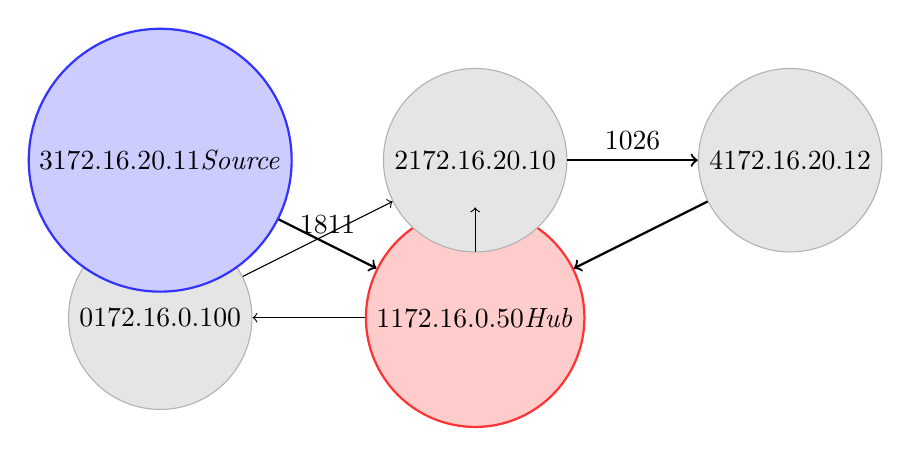
\begin{tikzpicture}[node distance=2cm, auto]
    % Define node styles
    \tikzstyle{hub} = [circle, draw=red!80, fill=red!20, thick, minimum size=1.5cm]
    \tikzstyle{source} = [circle, draw=blue!80, fill=blue!20, thick, minimum size=1.2cm]
    \tikzstyle{normal} = [circle, draw=gray!60, fill=gray!20, minimum size=1cm]
    
    % Nodes
    \node[normal] (n0) {0\\172.16.0.100};
    \node[hub] (n1) [right of=n0, xshift=2cm] {1\\172.16.0.50\\\textit{Hub}};
    \node[normal] (n2) [above of=n1] {2\\172.16.20.10};
    \node[source] (n3) [left of=n2, xshift=-2cm] {3\\172.16.20.11\\\textit{Source}};
    \node[normal] (n4) [right of=n2, xshift=2cm] {4\\172.16.20.12};
    
    % Edges (main connections)
    \draw[->, thick] (n3) -- node[above] {1811} (n1);
    \draw[->, thick] (n2) -- node[above] {1026} (n4);
    \draw[->, thick] (n4) -- (n1);
    \draw[->] (n1) -- (n0);
    \draw[->] (n0) -- (n2);
    \draw[->] (n2) -- (n1);
\end{tikzpicture}
\caption{Network structure of Global-APT dataset. Node 1 (172.16.0.50) acts as the central hub receiving 75\% of all connections. Node 3 (172.16.20.11) is the main source, sending 1,811 connections.}
\label{fig:network_structure}
\end{figure}

% ============================================================================
% FIGURE: Pipeline (convert Mermaid to TikZ or include as image)
% ============================================================================
\begin{figure}[htbp]
\centering
% Include pipeline diagram as image
% \includegraphics[width=\textwidth]{figures/pipeline.pdf}
\caption{Experimental pipeline: data preparation, temporal splitting, algorithm execution, and evaluation.}
\label{fig:pipeline}
\end{figure}

% ============================================================================
% DISCUSSION OF RESULTS
% ============================================================================
\subsection{Discussion}

The superior performance of GraphSAGE can be attributed to its ability to learn effective node embeddings by aggregating neighborhood information, which captures both local and global structural patterns. The automatic threshold optimization was crucial, as default thresholds led to overly conservative predictions.

The high recall but low precision of SLADE, GAT, and NetWalk suggests these methods are well-suited for scenarios where comprehensive anomaly detection is prioritized over precision. However, the large number of false positives (255-449) may limit their practical applicability without additional filtering mechanisms.

The poor performance of GeneralDYG highlights the importance of algorithm selection and hyperparameter tuning for specific dataset characteristics. Small, centralized graphs may require different approaches than large-scale distributed networks.

% ============================================================================
% STATISTICAL SIGNIFICANCE (optional)
% ============================================================================
% \subsection{Statistical Analysis}
% 
% We performed statistical significance tests to compare algorithm performance...
% (Add t-tests, confidence intervals, etc. if applicable)

% ============================================================================
% COMPUTATIONAL EFFICIENCY (optional)
% ============================================================================
% \subsection{Computational Efficiency}
% 
% Table~\ref{tab:efficiency} shows the training and inference times...
% (Add timing information if relevant for your paper)
